\chapter{Neutrino physics}
\label{sec:neutrino}

\epigraph{I have done a terrible thing, I have postulated a particle that cannot be detected.}{Wolfgang Pauli -- "Foreword" by Frederick Reines to "Spaceship Neutrino" by Christine Sutton, (p. xi), 1992. }

%\textit{In chapter 1, I'll remind briefly the SM, its limitations, and give a short introduction to neutrino physics, with a reminder of the present important questions and a state of the art.}


\minitoc

Our understanding of the universe describe it as composed of elementary components called elementary particles, the study of these particles is therefore particles physics. The theoretical model describing these particles and their interactions is the Standard Model (SM), with the exception of the gravitation. It has proven its robustness over the last decades, accounting for most of observed the phenomena with a few exception. This exception are phenomena described as Beyond Standard Model (BSM).

In this chapter in describe briefly the Standard model and its limitations in section \ref{sec:neutrinos:sm}, then delve a bit further in the specificity of neutrinos physics in Section \ref{sec:neutrino:th}.

\section{Introduction to the Standard model}
\label{sec:neutrinos:sm}

The SM categorize the elementary particles into two categories: the \textit{fermions} constituting the matter and the \textit{bosons} that mediate their interaction. The fermions are themselves divided in two categories, the \textit{quark} and the \textit{leptons}. Figure \ref{fig:neutrino:sm} shows the elementary particle and their classification. Each one these particle is characterized by the value of their quantum number the main one being their mass $m$, spin $J$ and electric charge $Q$. The leptons also possess leptonic quantum number $L = 1$ a flavor quantum number $L_{e,\mu,\tau}$ corresponding to their family, electronic, muonic or tauic. The leptons are thus split in three family: the electronic $L_e = 1 \rightarrow (e, \nu_e)$, muonic $L_\mu = 1 \rightarrow (\mu, \nu_\mu)$ and tauic $L_\tau = 1 \rightarrow (\tau, \nu_\tau)$ families, each composed of a charged $Q = 1$ and a neutral particle $Q = 0$. The neutral leptons are named the \textit{neutrinos} represented by the character $\nu$.

\begin{figure}
  \centering
  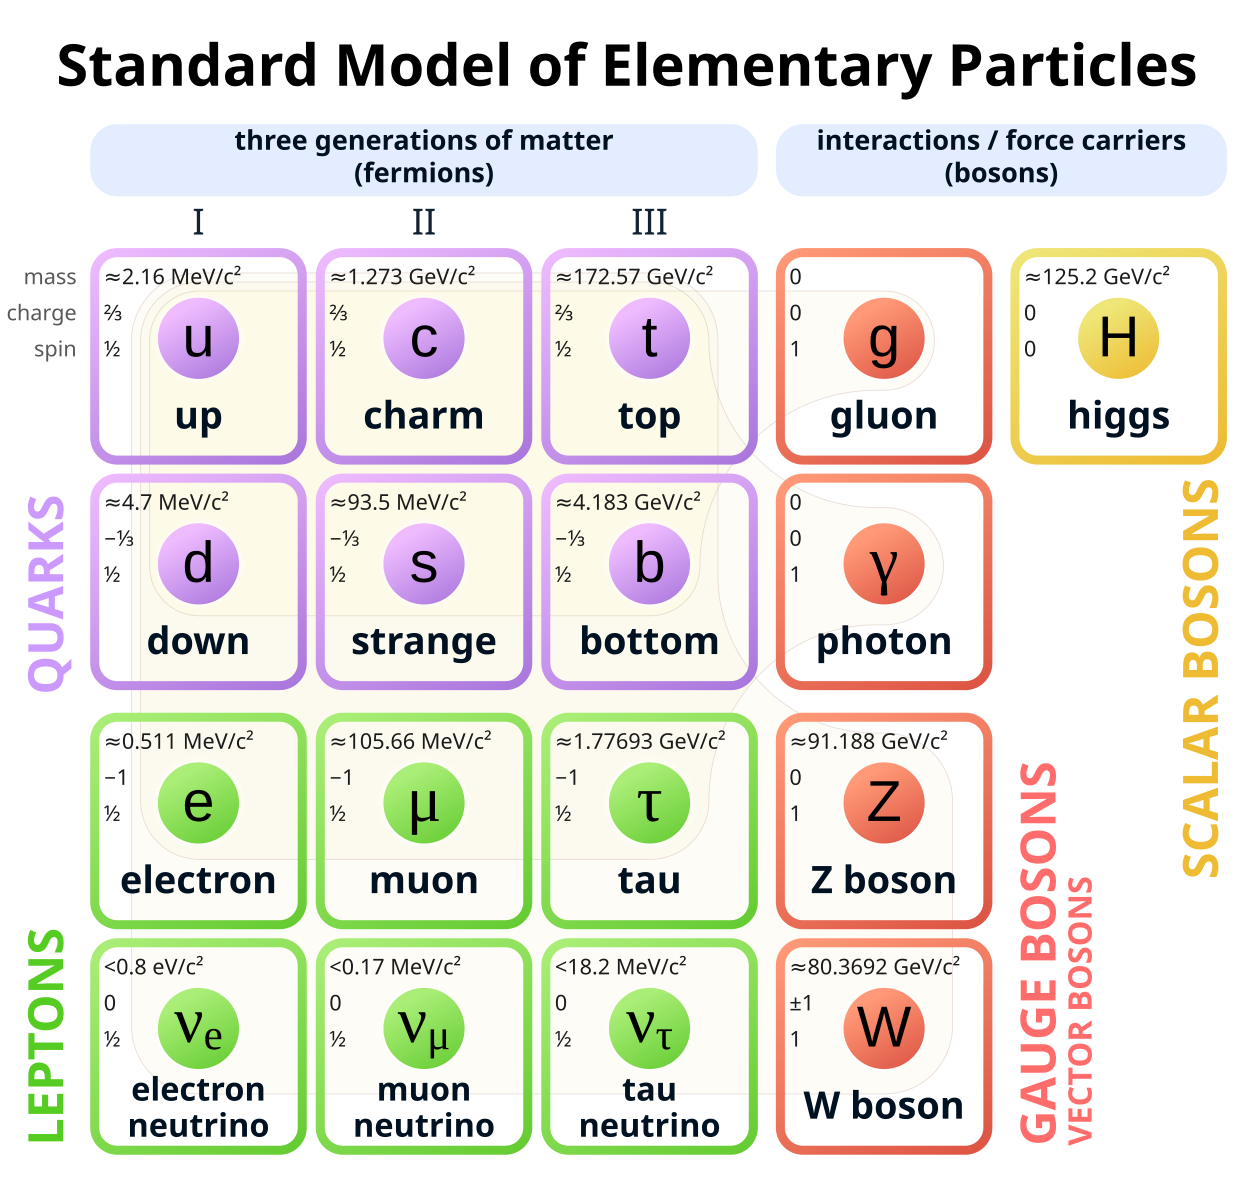
\includegraphics[height=6cm]{images/neutrinos/sm.png}
  \caption{List of the elementary particles in the Standard Model. The antiparticles are not displayed.}
  \label{fig:neutrino:sm}
\end{figure}

Each fermion also possess an antiparticle of opposite electric charge and opposite leptonic and flavour quantum number. Thus the antiparticle of the electron $e (Q=1, L=1, L_e=1)$, the positron is defined $e^+ (Q=-1, L=-1, L_e=-1)$.

The particles of the SM interact with each other via four interactions or forces. Three are described by the SM by the exchange of a boson:
\begin{itemize}
  \item The strong force, described by the exchange of a gluon. Only the quark are sensitive to it. This force is very small range $\sim 10^{-15}$ m, the size of a nucleus. It's the strong force that allow the cohesion of nucleus inside atoms. As its name indicates, it this the strongest of the four interaction.
  \item The electromagnetic force, described by the exchange of a photon. This force has unlimited range, all the charged particles -- quark and charged leptons -- are sensitive to it. It is responsible for every magnetic effect like the bonding of electrons and nucleus. Its relative strength with the strong force is 1/137.
  \item The weak force, carried by the $Z^0$ and $W^{\pm}$ bosons. Every fermions is sensitive to it. Its range is $\sim 10^{-18}$ m, $\sim 0.1\%$ the size of a proton. Its relative strength to the strong force is $10^{-6}$, explaining its name. It is responsible for nuclear beta decay and other similar process.
\end{itemize}

The final force, not described by the standard model, is the gravitational force. It's range is infinite, and concerns every massive ($m \neq 0$) particles. Its relative strength to the strong force is of $6\times 10^{-39}$. Extension to the SM propose a supplementary boson, the graviton, that be the carrier of the gravitational force but it has yet to be detected \cite{ParticleDataGroup:2024cfk, carney_graviton_2024}.

\subsubsection{Interactions and symmetries}

Symmetries are fundamental components of modern particle physics. As described in Noether's theorem \cite{noether_invariant_1971}, the invariance or non-invariance of the physics law under transformations (translation, rotation, ...), represented by the formal invariance of the SM Lagrangian ${\cal L}$ under those transformation, express the conservation of a quantity.

The invariance of ${\cal L}$ by translation in space characterize the conservation of the momentum, the rotational invariance in space the conservation of the angular momentum, the invariance by translation in time the conservation of energy, etc. If the transformation is continuous, the sum of the quantum numbers is conserved in a interaction.
Invariances under discrete transformation also provide conservation of quantum number. Three discrete transformations are important for the SM:
\begin{itemize}
  \item The parity $P$ symmetry transform $(\vec{x}, t) \rightarrow (-\vec{x}, t)$, reversing the handedness of space. The momentum thus become $\vec{p} \rightarrow -\vec{p}$ and the helicity $\frac{\vec{p} \cdot \vec{s}}{|\vec{p}|}$, where $\vec{s}$ is the spin, change sign.

  \item Reversal of time $T$ where $(\vec{x}, t) \rightarrow (\vec{x}, -t)$, inverting the initial and final state of an interaction $A + B \rightarrow C$ become $C \rightarrow A + B$. The momentum and the spin both change sign, leaving the helicity unchanged.

  \item Charge conjugation $C$, replacing the particles by their antiparticles counterpart and vice-versa, leaving untouched the momentum, spin and helicity.
\end{itemize}

The C, P and their combination CP symmetry was believed to be conserved until 1956, the discovery of their violation \cite{lee_question_1956, wu_experimental_1957, christenson_evidence_1964} in weak interaction revealed the non-triviality of its nature.

The fundamental symmetry CPT, the combination of C, P and T symmetry, is an exact symmetry. It mean that any process where the particles are switched with their anti-particles, spin-projection are of opposite sign and initial and final state are swapped must go with the same probability than the initial process. This implies that the mass, life times, absolute values of electric charge and magnetic moment of particles and antiparticles must be the same.

% Decrire le model standard -> Regarder theses LHC / Olga Kochebina

\subsection{Limits of the standard model}
% \marginpar{Limite du model standard - Interessant/justifier etudier les neutrinos -> violation de CP ? Pb des masses ?}
\section{The Neutrinos}
\label{sec:neutrino:th}

%\subsubsection{First theories}

%\subsubsection{Discovery}

%\subsubsection{Milestones and anomalies}

\subsection{Oscillation}
\label{sec:th:osc}

\subsection{Phenomenology}

\subsection{Open questions}
